
\documentclass{tufte-book}

%%% Disable auxiliary files
% These are used for references in latex documents, which are handled by
% disseminate. Additionally, aux files can trip up compiles of PDFs.
\nofiles

%%%
% Graphics
\usepackage{graphicx}

%%%
% Caption customization
\usepackage[labelformat=empty]{caption}

%%%
% title, section labels
\usepackage{titlesec}

%%%
% Panels for figures
\newenvironment{panel}[1]
{\begin{minipage}{ #1}\footnotesize}
{\end{minipage}}

%%%
% Load UTF-8 characters
% \usepackage[T1]{fontenc}  % introduces grainy bitmap fonts
\usepackage[utf8]{inputenc}
\DeclareUnicodeCharacter{26AC}{\circ}  % used for degrees
\DeclareUnicodeCharacter{25CB}{\ensuremath{\circ}}  % used for degrees
\DeclareUnicodeCharacter{00A7}{^^a7}

%%%
% Lists
\usepackage{easylist}

\usepackage{enumitem}
\setlistdepth{9}

%%%
% Math
\usepackage[fleqn]{amsmath}
\usepackage{mathtools}
\usepackage{bm}

%%%
% Hyperref package for links
\usepackage{hyperref}
\hypersetup{ %colorlinks,
            %linkcolor=black!50!blue,
            %filecolor=black!50!blue,pdftitle=Fundamentals of NMR Spectroscopy,pdfauthor=Justin Lorieau,
            pdfcreator=Disseminate
            }

%%%
% Page Layout
\usepackage{geometry}
% Increase text height and bottom margin
\geometry{
  textheight=48\baselineskip,
  textwidth=114mm, % main text block
  marginparsep=8mm, % gutter between main text block and margin notes
  marginparwidth=55mm, % width of margin notes
}
\setlength{\evensidemargin}{-0.5in}

%%%
% Colors
\usepackage{xcolor}

%%%
% Counters
\newcounter{title}

%%% 
% Symbols
\renewcommand{\deg}{^\circ}

%%%
% Nice tables
\usepackage{booktabs}

%%%
% Color boxes
\usepackage[breakable]{tcolorbox}

\newtcolorbox{featurebox}{colback=black!5!white,
                          colframe=black!40!white,
                          breakable,
                          before skip=\baselineskip,
                          after skip=\baselineskip}
\newtcolorbox{examplebox}{colback=blue!5!white,
                          colframe=blue!40!white,
                          breakable,
                          before skip=\baselineskip,
                          after skip=\baselineskip}
\newtcolorbox{problembox}{colback=green!7!white,
                          colframe=green!50!black!40!white,
                          breakable,
                          before skip=\baselineskip,
                          after skip=\baselineskip}
\usepackage{fancyvrb}

\makeatletter
\def\PY@reset{\let\PY@it=\relax \let\PY@bf=\relax%
    \let\PY@ul=\relax \let\PY@tc=\relax%
    \let\PY@bc=\relax \let\PY@ff=\relax}
\def\PY@tok#1{\csname PY@tok@#1\endcsname}
\def\PY@toks#1+{\ifx\relax#1\empty\else%
    \PY@tok{#1}\expandafter\PY@toks\fi}
\def\PY@do#1{\PY@bc{\PY@tc{\PY@ul{%
    \PY@it{\PY@bf{\PY@ff{#1}}}}}}}
\def\PY#1#2{\PY@reset\PY@toks#1+\relax+\PY@do{#2}}

\expandafter\def\csname PY@tok@w\endcsname{\def\PY@tc##1{\textcolor[rgb]{0.73,0.73,0.73}{##1}}}
\expandafter\def\csname PY@tok@c\endcsname{\let\PY@it=\textit\def\PY@tc##1{\textcolor[rgb]{0.25,0.50,0.50}{##1}}}
\expandafter\def\csname PY@tok@cp\endcsname{\def\PY@tc##1{\textcolor[rgb]{0.74,0.48,0.00}{##1}}}
\expandafter\def\csname PY@tok@k\endcsname{\let\PY@bf=\textbf\def\PY@tc##1{\textcolor[rgb]{0.00,0.50,0.00}{##1}}}
\expandafter\def\csname PY@tok@kp\endcsname{\def\PY@tc##1{\textcolor[rgb]{0.00,0.50,0.00}{##1}}}
\expandafter\def\csname PY@tok@kt\endcsname{\def\PY@tc##1{\textcolor[rgb]{0.69,0.00,0.25}{##1}}}
\expandafter\def\csname PY@tok@o\endcsname{\def\PY@tc##1{\textcolor[rgb]{0.40,0.40,0.40}{##1}}}
\expandafter\def\csname PY@tok@ow\endcsname{\let\PY@bf=\textbf\def\PY@tc##1{\textcolor[rgb]{0.67,0.13,1.00}{##1}}}
\expandafter\def\csname PY@tok@nb\endcsname{\def\PY@tc##1{\textcolor[rgb]{0.00,0.50,0.00}{##1}}}
\expandafter\def\csname PY@tok@nf\endcsname{\def\PY@tc##1{\textcolor[rgb]{0.00,0.00,1.00}{##1}}}
\expandafter\def\csname PY@tok@nc\endcsname{\let\PY@bf=\textbf\def\PY@tc##1{\textcolor[rgb]{0.00,0.00,1.00}{##1}}}
\expandafter\def\csname PY@tok@nn\endcsname{\let\PY@bf=\textbf\def\PY@tc##1{\textcolor[rgb]{0.00,0.00,1.00}{##1}}}
\expandafter\def\csname PY@tok@ne\endcsname{\let\PY@bf=\textbf\def\PY@tc##1{\textcolor[rgb]{0.82,0.25,0.23}{##1}}}
\expandafter\def\csname PY@tok@nv\endcsname{\def\PY@tc##1{\textcolor[rgb]{0.10,0.09,0.49}{##1}}}
\expandafter\def\csname PY@tok@no\endcsname{\def\PY@tc##1{\textcolor[rgb]{0.53,0.00,0.00}{##1}}}
\expandafter\def\csname PY@tok@nl\endcsname{\def\PY@tc##1{\textcolor[rgb]{0.63,0.63,0.00}{##1}}}
\expandafter\def\csname PY@tok@ni\endcsname{\let\PY@bf=\textbf\def\PY@tc##1{\textcolor[rgb]{0.60,0.60,0.60}{##1}}}
\expandafter\def\csname PY@tok@na\endcsname{\def\PY@tc##1{\textcolor[rgb]{0.49,0.56,0.16}{##1}}}
\expandafter\def\csname PY@tok@nt\endcsname{\let\PY@bf=\textbf\def\PY@tc##1{\textcolor[rgb]{0.00,0.50,0.00}{##1}}}
\expandafter\def\csname PY@tok@nd\endcsname{\def\PY@tc##1{\textcolor[rgb]{0.67,0.13,1.00}{##1}}}
\expandafter\def\csname PY@tok@s\endcsname{\def\PY@tc##1{\textcolor[rgb]{0.73,0.13,0.13}{##1}}}
\expandafter\def\csname PY@tok@sd\endcsname{\let\PY@it=\textit\def\PY@tc##1{\textcolor[rgb]{0.73,0.13,0.13}{##1}}}
\expandafter\def\csname PY@tok@si\endcsname{\let\PY@bf=\textbf\def\PY@tc##1{\textcolor[rgb]{0.73,0.40,0.53}{##1}}}
\expandafter\def\csname PY@tok@se\endcsname{\let\PY@bf=\textbf\def\PY@tc##1{\textcolor[rgb]{0.73,0.40,0.13}{##1}}}
\expandafter\def\csname PY@tok@sr\endcsname{\def\PY@tc##1{\textcolor[rgb]{0.73,0.40,0.53}{##1}}}
\expandafter\def\csname PY@tok@ss\endcsname{\def\PY@tc##1{\textcolor[rgb]{0.10,0.09,0.49}{##1}}}
\expandafter\def\csname PY@tok@sx\endcsname{\def\PY@tc##1{\textcolor[rgb]{0.00,0.50,0.00}{##1}}}
\expandafter\def\csname PY@tok@m\endcsname{\def\PY@tc##1{\textcolor[rgb]{0.40,0.40,0.40}{##1}}}
\expandafter\def\csname PY@tok@gh\endcsname{\let\PY@bf=\textbf\def\PY@tc##1{\textcolor[rgb]{0.00,0.00,0.50}{##1}}}
\expandafter\def\csname PY@tok@gu\endcsname{\let\PY@bf=\textbf\def\PY@tc##1{\textcolor[rgb]{0.50,0.00,0.50}{##1}}}
\expandafter\def\csname PY@tok@gd\endcsname{\def\PY@tc##1{\textcolor[rgb]{0.63,0.00,0.00}{##1}}}
\expandafter\def\csname PY@tok@gi\endcsname{\def\PY@tc##1{\textcolor[rgb]{0.00,0.63,0.00}{##1}}}
\expandafter\def\csname PY@tok@gr\endcsname{\def\PY@tc##1{\textcolor[rgb]{1.00,0.00,0.00}{##1}}}
\expandafter\def\csname PY@tok@ge\endcsname{\let\PY@it=\textit}
\expandafter\def\csname PY@tok@gs\endcsname{\let\PY@bf=\textbf}
\expandafter\def\csname PY@tok@gp\endcsname{\let\PY@bf=\textbf\def\PY@tc##1{\textcolor[rgb]{0.00,0.00,0.50}{##1}}}
\expandafter\def\csname PY@tok@go\endcsname{\def\PY@tc##1{\textcolor[rgb]{0.53,0.53,0.53}{##1}}}
\expandafter\def\csname PY@tok@gt\endcsname{\def\PY@tc##1{\textcolor[rgb]{0.00,0.27,0.87}{##1}}}
\expandafter\def\csname PY@tok@err\endcsname{\def\PY@bc##1{\setlength{\fboxsep}{0pt}\fcolorbox[rgb]{1.00,0.00,0.00}{1,1,1}{\strut ##1}}}
\expandafter\def\csname PY@tok@kc\endcsname{\let\PY@bf=\textbf\def\PY@tc##1{\textcolor[rgb]{0.00,0.50,0.00}{##1}}}
\expandafter\def\csname PY@tok@kd\endcsname{\let\PY@bf=\textbf\def\PY@tc##1{\textcolor[rgb]{0.00,0.50,0.00}{##1}}}
\expandafter\def\csname PY@tok@kn\endcsname{\let\PY@bf=\textbf\def\PY@tc##1{\textcolor[rgb]{0.00,0.50,0.00}{##1}}}
\expandafter\def\csname PY@tok@kr\endcsname{\let\PY@bf=\textbf\def\PY@tc##1{\textcolor[rgb]{0.00,0.50,0.00}{##1}}}
\expandafter\def\csname PY@tok@bp\endcsname{\def\PY@tc##1{\textcolor[rgb]{0.00,0.50,0.00}{##1}}}
\expandafter\def\csname PY@tok@fm\endcsname{\def\PY@tc##1{\textcolor[rgb]{0.00,0.00,1.00}{##1}}}
\expandafter\def\csname PY@tok@vc\endcsname{\def\PY@tc##1{\textcolor[rgb]{0.10,0.09,0.49}{##1}}}
\expandafter\def\csname PY@tok@vg\endcsname{\def\PY@tc##1{\textcolor[rgb]{0.10,0.09,0.49}{##1}}}
\expandafter\def\csname PY@tok@vi\endcsname{\def\PY@tc##1{\textcolor[rgb]{0.10,0.09,0.49}{##1}}}
\expandafter\def\csname PY@tok@vm\endcsname{\def\PY@tc##1{\textcolor[rgb]{0.10,0.09,0.49}{##1}}}
\expandafter\def\csname PY@tok@sa\endcsname{\def\PY@tc##1{\textcolor[rgb]{0.73,0.13,0.13}{##1}}}
\expandafter\def\csname PY@tok@sb\endcsname{\def\PY@tc##1{\textcolor[rgb]{0.73,0.13,0.13}{##1}}}
\expandafter\def\csname PY@tok@sc\endcsname{\def\PY@tc##1{\textcolor[rgb]{0.73,0.13,0.13}{##1}}}
\expandafter\def\csname PY@tok@dl\endcsname{\def\PY@tc##1{\textcolor[rgb]{0.73,0.13,0.13}{##1}}}
\expandafter\def\csname PY@tok@s2\endcsname{\def\PY@tc##1{\textcolor[rgb]{0.73,0.13,0.13}{##1}}}
\expandafter\def\csname PY@tok@sh\endcsname{\def\PY@tc##1{\textcolor[rgb]{0.73,0.13,0.13}{##1}}}
\expandafter\def\csname PY@tok@s1\endcsname{\def\PY@tc##1{\textcolor[rgb]{0.73,0.13,0.13}{##1}}}
\expandafter\def\csname PY@tok@mb\endcsname{\def\PY@tc##1{\textcolor[rgb]{0.40,0.40,0.40}{##1}}}
\expandafter\def\csname PY@tok@mf\endcsname{\def\PY@tc##1{\textcolor[rgb]{0.40,0.40,0.40}{##1}}}
\expandafter\def\csname PY@tok@mh\endcsname{\def\PY@tc##1{\textcolor[rgb]{0.40,0.40,0.40}{##1}}}
\expandafter\def\csname PY@tok@mi\endcsname{\def\PY@tc##1{\textcolor[rgb]{0.40,0.40,0.40}{##1}}}
\expandafter\def\csname PY@tok@il\endcsname{\def\PY@tc##1{\textcolor[rgb]{0.40,0.40,0.40}{##1}}}
\expandafter\def\csname PY@tok@mo\endcsname{\def\PY@tc##1{\textcolor[rgb]{0.40,0.40,0.40}{##1}}}
\expandafter\def\csname PY@tok@ch\endcsname{\let\PY@it=\textit\def\PY@tc##1{\textcolor[rgb]{0.25,0.50,0.50}{##1}}}
\expandafter\def\csname PY@tok@cm\endcsname{\let\PY@it=\textit\def\PY@tc##1{\textcolor[rgb]{0.25,0.50,0.50}{##1}}}
\expandafter\def\csname PY@tok@cpf\endcsname{\let\PY@it=\textit\def\PY@tc##1{\textcolor[rgb]{0.25,0.50,0.50}{##1}}}
\expandafter\def\csname PY@tok@c1\endcsname{\let\PY@it=\textit\def\PY@tc##1{\textcolor[rgb]{0.25,0.50,0.50}{##1}}}
\expandafter\def\csname PY@tok@cs\endcsname{\let\PY@it=\textit\def\PY@tc##1{\textcolor[rgb]{0.25,0.50,0.50}{##1}}}

\def\PYZbs{\char`\\}
\def\PYZus{\char`\_}
\def\PYZob{\char`\{}
\def\PYZcb{\char`\}}
\def\PYZca{\char`\^}
\def\PYZam{\char`\&}
\def\PYZlt{\char`\<}
\def\PYZgt{\char`\>}
\def\PYZsh{\char`\#}
\def\PYZpc{\char`\%}
\def\PYZdl{\char`\$}
\def\PYZhy{\char`\-}
\def\PYZsq{\char`\'}
\def\PYZdq{\char`\"}
\def\PYZti{\char`\~}
% for compatibility with earlier versions
\def\PYZat{@}
\def\PYZlb{[}
\def\PYZrb{]}
\makeatother
%%%
% Remove labels from captions  
\usepackage{etoolbox}
\makeatletter
\patchcmd{\@caption}
  {\noindent\csname fnum@#1\endcsname: \ignorespaces}
  {\noindent}
  {}{}
\makeatother

%%%
% Format chapter headings
\usepackage[Bjornstrup]{fncychap}
\setcounter{secnumdepth}{0} % turn on numbering for parts and chapters
\title{
        Fundamentals of NMR Spectroscopy
    }
    \author{
        Justin Lorieau
    }

\begin{document}
\mainmatter  % Needed to set chapter/section numbering
\setcounter{chapter}{0}
\chapter{INEPT and Signal Enhancement} \label{ch:fundamental-solnnmr-inept-inept-dm-inept-and-signal-enhancement}

Justin Lorieau

The purpose of the INEPT sequence \marginnote{Morris GA, Freeman
R. Enhancement of Nuclear Magnetic Resonance Signals by Polarization
Transfer. J Am Chem Soc. 1979;101(3):760–762.} is to transfer the
large magnetization from high-\ensuremath{\gamma} nuclei, like \ensuremath{^{1}}H or \ensuremath{^{19}}F, to
low-\ensuremath{\gamma} nuclei (labeled ‘X’), like \ensuremath{^{13}}C and \ensuremath{^{15}}N. This transfer
significantly improves the signal intensity of ‘X’ nuclei when
measuring their chemical shifts. For example, the magnetic moment and
magnetization of \ensuremath{^{1}}H nuclei is roughly 4 times greater than \ensuremath{^{13}}C and
10 times greater than \ensuremath{^{15}}N. Additionally, the \ensuremath{^{1}}H T\ensuremath{_{1}} is typically
much shorter than the T\ensuremath{_{1}} for \ensuremath{^{13}}C or \ensuremath{^{15}}N, which allows a shorter
recycle delay and the collection of a greater number of spectra.
\setcounter{section}{0}
\section{1.1. Theory} \label{sec:fundamental-solnnmr-inept-inept-dm-theory}
\begin{marginfigure}
  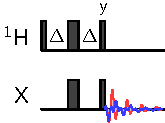
\includegraphics{{tex/media/inept_28e2ce5d5bc5}.pdf}
  \caption{\textbf{Fig. 1.1}. The basic INEPT sequence between nuclei \ensuremath{^{1}}H
    and X.} \label{fig:inept-inept1}
\end{marginfigure}

The INEPT sequence (\href{#fig:inept-inept1}{Fig. 1.1}) transfers
magnetization from \ensuremath{^{1}}H nuclei bonded the ‘X’ nuclei. The two
nuclei must be bonded, or at least connected through intermediary
bonds with other atoms, because the nuclei must share a J-coupling.

The INEPT sequence comprises a set of 90\ensuremath{^{○}} pulses (thin bars),
180\ensuremath{^{○}} pulses (thick bars) and delays (\ensuremath{\Delta}).
\setcounter{subsection}{0}
\subsection{1.1.1. Methine, Amide and the AX Spin Systems} \label{subsec:fundamental-solnnmr-inept-inept-dm-methine-amide-and-the-ax-spin-systems}
The first 90\ensuremath{^{○}_{x}} (\ensuremath{^{1}}H) pulse creates \ensuremath{\boldsymbol{-H_y}} \ensuremath{^{1}}H magnetization.
\marginnote{A 90\ensuremath{^{○}_{x}} pulse rotates the magnetization by 90\ensuremath{^{○}} with a phase
of ‘x’.}  Thereafter, the \ensuremath{^{1}}H 180\ensuremath{^{○}} pulse in the middle of the two
\ensuremath{\Delta} delays acts as a Hahn-echo to refocus the \ensuremath{^{1}}H chemical
shifts. Without the accompanying 180\ensuremath{^{○}} pulse on the ‘X’ channel, the
J-coupling between the \ensuremath{^{1}}H and X nucleus would be refocused as
well—and nothing would be accomplished. The 180\ensuremath{^{○}} pulse on the ‘X’
channel acts to \textit{cancel} the refocusing effect of the \ensuremath{^{1}}H 180\ensuremath{^{○}}
pulse for the J-coupling.

During the first delta period, the \ensuremath{\boldsymbol{- H_y}} magnetization evolves
under the \ensuremath{^{1}}H chemical shift (\ensuremath{\omega}\ensuremath{_{H}}) and the \ensuremath{^{1}}H-X
J-coupling. Since the chemical shift and J-coupling Hamiltonians
commute, the rotations of each can be conducted sequentially.

In the first step, the operators are propagated for the 90\ensuremath{^{○}_{x}} (\ensuremath{^{1}}H) pulse
and the first '\ensuremath{\Delta}' period. We’ll use a \ensuremath{^{15}}N nucleus as an example
of an ‘X’ nucleus.

\begin{marginfigure}
  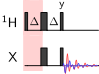
\includegraphics{{tex/media/inept_750faf39a819}.pdf}
  \caption{\textbf{Fig. 1.2}. The first step of the INEPT sequence highlighted in
    red.} \label{caption-e094a2f6ff}
  
\end{marginfigure}
\begin{alignat*}{3} %
\boldsymbol{H_z} & \xrightarrow{\mathmakebox[3em]{90^{○}_{x} (^{1}H)}} && \boldsymbol{- H_y} \\
  \boldsymbol{-H_y}& \xrightarrow{\mathmakebox[3em]{\omega_{H}\Delta}} &&
    \boldsymbol{-H_y} \cos(\omega_{H} \Delta) + \boldsymbol{H_x} \sin(\omega_{H} \Delta) \\
  & \xrightarrow{\mathmakebox[3em]{J_{NH} \Delta}} &&
  \boldsymbol{-H_y} \cos(\omega_{H} \Delta) \cos(\pi J_{NH} \Delta) + \\
   & &&
  \quad \boldsymbol{2H_x N_z} \cos(\omega_{H} \Delta) \sin(\pi J_{NH} \Delta) + \\
   & &&
  \quad \boldsymbol{H_x} \sin(\omega_{H} \Delta) \cos(\pi J_{NH} \Delta) + \\
   & &&
  \quad \boldsymbol{2H_y N_z} \sin(\omega_{H} \Delta) \sin(\pi J_{NH} \Delta)
\end{alignat*}
In the second step, the 180\ensuremath{^{○}_{x}} pulses on the \ensuremath{^{1}}H and
‘X’ channels inverts \ensuremath{\boldsymbol{H_y}} and \ensuremath{\boldsymbol{2H_x N_z}} terms because
these are orthogonal to the x-phase of the pulse.\marginnote{
The many cosine and sine terms can be abbreviated to simplify
  their notation in equations.
  \begin{align*} %
\cos(\omega_{H} \Delta) &= \textcolor{blue}{C_{CS\Delta}} \\
  \cos(\pi J_{NH} \Delta) &= \textcolor{blue}{C_{J_{NH} \Delta}} \\
  \sin(\omega_{H} \Delta) &= \textcolor{red!80!black}{S_{CS\Delta}} \\
  \sin(\pi J_{NH} \Delta) &= \textcolor{red!80!black}{S_{J_{NH} \Delta}}
\end{align*}
}

\begin{marginfigure}
  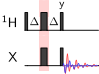
\includegraphics{{tex/media/inept_863891104408}.pdf}
    \caption{\textbf{Fig. 1.3}. The second step of the INEPT sequence highlighted in
  red.} \label{caption-4309bc4697}
  
\end{marginfigure}
\begin{align*} %
\xrightarrow{\mathmakebox[6em]{180^{○}_{x} (^{1}H),\ 180^{○}_{x} (X)}}
   &
   \quad \boldsymbol{H_y} \textcolor{blue}{C_{CS\Delta}} \textcolor{blue}{C_{J_{NH} \Delta}} - \boldsymbol{2H_x N_z} \textcolor{blue}{C_{CS\Delta}} \textcolor{red!80!black}{S_{J_{NH} \Delta}} \\
   &
   + \boldsymbol{H_x} \textcolor{blue}{C_{CS\Delta}} \textcolor{blue}{C_{J_{NH} \Delta}} + \boldsymbol{2H_y N_z} \textcolor{red!80!black}{S_{CS\Delta}} \textcolor{red!80!black}{S_{J_{NH} \Delta}}
&
\end{align*}
In the third step, we’ll propagate the `\ensuremath{\Delta}' delay for the chemical shift
first.

\begin{marginfigure}
  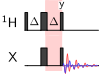
\includegraphics{{tex/media/inept_3a2decf4b06c}.pdf}
  \caption{\textbf{Fig. 1.4}. The third step of the INEPT sequence highlighted in
    red.} \label{caption-b5c24eb647}
\end{marginfigure}
\begin{align*} %
\xrightarrow{\mathmakebox[2em]{\omega_{H} \Delta}}
 &
 \quad \boldsymbol{H_y} \textcolor{blue}{C_{CS\Delta}} \textcolor{blue}{C_{J_{NH} \Delta}} \textcolor{blue}{C_{CS\Delta}}
       -H_x \textcolor{blue}{C_{CS\Delta}} \textcolor{blue}{C_{J_{NH} \Delta}} \textcolor{red!80!black}{S_{CS\Delta}} \\
 &
       \boldsymbol{-2H_x N_z} \textcolor{blue}{C_{CS\Delta}} \textcolor{red!80!black}{S_{J_{NH} \Delta}} \textcolor{blue}{C_{CS\Delta}}
       \boldsymbol{-2H_y N_z} \textcolor{blue}{C_{CS\Delta}} \textcolor{red!80!black}{S_{J_{NH} \Delta}} \textcolor{red!80!black}{S_{CS\Delta}} \\
  &
 \quad \boldsymbol{H_x} \textcolor{red!80!black}{S_{CS\Delta}} \textcolor{blue}{C_{J_{NH} \Delta}} \textcolor{blue}{C_{CS\Delta}}  +
       \boldsymbol{H_y} \textcolor{red!80!black}{S_{CS\Delta}} \textcolor{blue}{C_{J_{NH} \Delta}} \textcolor{red!80!black}{S_{CS\Delta}}  + \\
 &
 \quad \boldsymbol{2H_y N_z} \textcolor{red!80!black}{S_{CS\Delta}} \textcolor{red!80!black}{S_{J_{NH} \Delta}} \textcolor{blue}{C_{CS\Delta}} +
       \boldsymbol{-2H_x N_z} \textcolor{red!80!black}{S_{CS\Delta}} \textcolor{red!80!black}{S_{J_{NH} \Delta}} \textcolor{red!80!black}{S_{CS\Delta}}
\end{align*}
These terms can be grouped.
\begin{align*} %
=& \quad \boldsymbol{H_x} (\textcolor{red!80!black}{S_{CS\Delta}} \textcolor{blue}{C_{J_{NH} \Delta}} \textcolor{blue}{C_{CS\Delta}} - \textcolor{blue}{C_{CS\Delta}} \textcolor{blue}{C_{J_{NH} \Delta}} \textcolor{red!80!black}{S_{CS\Delta}}) \\
  &      + \boldsymbol{H_y} (\textcolor{blue}{C_{CS\Delta}} \textcolor{blue}{C_{J_{NH} \Delta}} \textcolor{blue}{C_{CS\Delta}} + \textcolor{red!80!black}{S_{CS\Delta}} \textcolor{blue}{C_{J_{NH} \Delta}} \textcolor{red!80!black}{S_{CS\Delta}})  \\
  &      - \boldsymbol{2H_x N_z} (\textcolor{blue}{C_{CS\Delta}} \textcolor{red!80!black}{S_{J_{NH} \Delta}} \textcolor{blue}{C_{CS\Delta}} + \textcolor{red!80!black}{S_{CS\Delta}} \textcolor{red!80!black}{S_{J_{NH} \Delta}} \textcolor{red!80!black}{S_{CS\Delta}}) \\
  &      + \boldsymbol{2H_y N_z} (\textcolor{red!80!black}{S_{CS\Delta}} \textcolor{red!80!black}{S_{J_{NH} \Delta}} \textcolor{blue}{C_{CS\Delta}} - \textcolor{blue}{C_{CS\Delta}} \textcolor{red!80!black}{S_{J_{NH} \Delta}} \textcolor{red!80!black}{S_{CS\Delta}})
\end{align*}
Thereafter, we propagate the '\ensuremath{\Delta}' delay for the J\ensuremath{_{NH}}-coupling and simplify the expression.

\begin{align*} %
\xrightarrow{\mathmakebox[2em]{J_{NH} \Delta}}
 & \quad \boldsymbol{H_x} (\textcolor{red!80!black}{S_{CS\Delta}} \textcolor{blue}{C_{J_{NH} \Delta}} \textcolor{blue}{C_{CS\Delta}} -
                      \textcolor{blue}{C_{CS\Delta}} \textcolor{blue}{C_{J_{NH} \Delta}} \textcolor{red!80!black}{S_{CS\Delta}}) \textcolor{blue}{C_{J_{NH} \Delta}}  \\
 &     + \boldsymbol{2 H_y N_z} (\textcolor{red!80!black}{S_{CS\Delta}} \textcolor{blue}{C_{J_{NH} \Delta}} \textcolor{blue}{C_{CS\Delta}} -
                            \textcolor{blue}{C_{CS\Delta}} \textcolor{blue}{C_{J_{NH} \Delta}} \textcolor{red!80!black}{S_{CS\Delta}}) \textcolor{red!80!black}{S_{J_{NH} \Delta}} \\
 &     + \boldsymbol{H_y} (\textcolor{blue}{C_{CS\Delta}} \textcolor{blue}{C_{J_{NH} \Delta}} \textcolor{blue}{C_{CS\Delta}} +
                      \textcolor{red!80!black}{S_{CS\Delta}} \textcolor{blue}{C_{J_{NH} \Delta}} \textcolor{red!80!black}{S_{CS\Delta}}) \textcolor{blue}{C_{J_{NH} \Delta}} \\
 &     - \boldsymbol{2H_x N_z} (\textcolor{blue}{C_{CS\Delta}} \textcolor{blue}{C_{J_{NH} \Delta}} \textcolor{blue}{C_{CS\Delta}} +
                           \textcolor{red!80!black}{S_{CS\Delta}} \textcolor{blue}{C_{J_{NH} \Delta}} \textcolor{red!80!black}{S_{CS\Delta}}) \textcolor{red!80!black}{S_{J_{NH} \Delta}} \\
 &     - \boldsymbol{2H_x N_z} (\textcolor{blue}{C_{CS\Delta}} \textcolor{red!80!black}{S_{J_{NH} \Delta}} \textcolor{blue}{C_{CS\Delta}} +
                           \textcolor{red!80!black}{S_{CS\Delta}} \textcolor{red!80!black}{S_{J_{NH} \Delta}} \textcolor{red!80!black}{S_{CS\Delta}}) \textcolor{blue}{C_{J_{NH} \Delta}} \\
 &     - \boldsymbol{H_y} (\textcolor{blue}{C_{CS\Delta}} \textcolor{red!80!black}{S_{J_{NH} \Delta}} \textcolor{blue}{C_{CS\Delta}} +
                      \textcolor{red!80!black}{S_{CS\Delta}} \textcolor{red!80!black}{S_{J_{NH} \Delta}} \textcolor{red!80!black}{S_{CS\Delta}}) \textcolor{red!80!black}{S_{J_{NH} \Delta}} \\
 &     + \boldsymbol{2H_y N_z} (\textcolor{red!80!black}{S_{CS\Delta}} \textcolor{red!80!black}{S_{J_{NH} \Delta}} \textcolor{blue}{C_{CS\Delta}} -
                           \textcolor{blue}{C_{CS\Delta}} \textcolor{red!80!black}{S_{J_{NH} \Delta}} \textcolor{red!80!black}{S_{CS\Delta}}) \textcolor{blue}{C_{J_{NH} \Delta}} \\
 &     - \boldsymbol{H_x} (\textcolor{red!80!black}{S_{CS\Delta}} \textcolor{red!80!black}{S_{J_{NH} \Delta}} \textcolor{blue}{C_{CS\Delta}} -
                      \textcolor{blue}{C_{CS\Delta}} \textcolor{red!80!black}{S_{J_{NH} \Delta}} \textcolor{red!80!black}{S_{CS\Delta}}) \textcolor{red!80!black}{S_{J_{NH} \Delta}} \displaybreak[2] \\[0.5em]
  =
  & \quad \boldsymbol{H_x} (\textcolor{red!80!black}{S_{CS\Delta}} \textcolor{blue}{C_{J_{NH} \Delta}} \textcolor{blue}{C_{CS\Delta}} \textcolor{blue}{C_{J_{NH} \Delta}} - \textcolor{blue}{C_{CS\Delta}} \textcolor{blue}{C_{J_{NH} \Delta}} \textcolor{red!80!black}{S_{CS\Delta}} \textcolor{blue}{C_{J_{NH} \Delta}} \\
  &                    - \textcolor{red!80!black}{S_{CS\Delta}} \textcolor{red!80!black}{S_{J_{NH} \Delta}} \textcolor{blue}{C_{CS\Delta}} \textcolor{red!80!black}{S_{J_{NH} \Delta}} + \textcolor{blue}{C_{CS\Delta}} \textcolor{red!80!black}{S_{J_{NH} \Delta}} \textcolor{red!80!black}{S_{CS\Delta}} \textcolor{red!80!black}{S_{J_{NH} \Delta}} ) \\
  & \quad \boldsymbol{H_y} (\textcolor{blue}{C_{CS\Delta}} \textcolor{blue}{C_{J_{NH} \Delta}} \textcolor{blue}{C_{CS\Delta}} \textcolor{blue}{C_{J_{NH} \Delta}} + \textcolor{red!80!black}{S_{CS\Delta}} \textcolor{blue}{C_{J_{NH} \Delta}} \textcolor{red!80!black}{S_{CS\Delta}} \textcolor{blue}{C_{J_{NH} \Delta}} \\
  &                    - \textcolor{blue}{C_{CS\Delta}} \textcolor{red!80!black}{S_{J_{NH} \Delta}} \textcolor{blue}{C_{CS\Delta}} \textcolor{red!80!black}{S_{J_{NH} \Delta}} - \textcolor{red!80!black}{S_{CS\Delta}} \textcolor{red!80!black}{S_{J_{NH} \Delta}} \textcolor{red!80!black}{S_{CS\Delta}} \textcolor{red!80!black}{S_{J_{NH} \Delta}}) \\
  &       \boldsymbol{-2 H_x N_z} (\textcolor{blue}{C_{CS\Delta}} \textcolor{blue}{C_{J_{NH} \Delta}} \textcolor{blue}{C_{CS\Delta}} \textcolor{red!80!black}{S_{J_{NH} \Delta}} + \textcolor{red!80!black}{S_{CS\Delta}} \textcolor{blue}{C_{J_{NH} \Delta}} \textcolor{red!80!black}{S_{CS\Delta}} \textcolor{red!80!black}{S_{J_{NH} \Delta}} \\
  &                           + \textcolor{blue}{C_{CS\Delta}} \textcolor{red!80!black}{S_{J_{NH} \Delta}} \textcolor{blue}{C_{CS\Delta}} \textcolor{blue}{C_{J_{NH} \Delta}} + \textcolor{red!80!black}{S_{CS\Delta}} \textcolor{red!80!black}{S_{J_{NH} \Delta}} \textcolor{red!80!black}{S_{CS\Delta}} \textcolor{blue}{C_{J_{NH} \Delta}}) \\
  & \quad \boldsymbol{2 H_y N_z} (\textcolor{red!80!black}{S_{CS\Delta}} \textcolor{blue}{C_{J_{NH} \Delta}} \textcolor{blue}{C_{CS\Delta}} \textcolor{red!80!black}{S_{J_{NH} \Delta}} - \textcolor{blue}{C_{CS\Delta}} \textcolor{blue}{C_{J_{NH} \Delta}} \textcolor{red!80!black}{S_{CS\Delta}} \textcolor{red!80!black}{S_{J_{NH} \Delta}} \\
  &                          + \textcolor{red!80!black}{S_{CS\Delta}} \textcolor{red!80!black}{S_{J_{NH} \Delta}} \textcolor{blue}{C_{CS\Delta}} \textcolor{blue}{C_{J_{NH} \Delta}} - \textcolor{blue}{C_{CS\Delta}} \textcolor{red!80!black}{S_{J_{NH} \Delta}} \textcolor{red!80!black}{S_{CS\Delta}} \textcolor{blue}{C_{J_{NH} \Delta}}) \displaybreak[2] \\[0.5em]
  =
  &       \boldsymbol{-2 H_x N_z} \sin(2 \pi J_{NH} \Delta) + \boldsymbol{H_y} \cos(2 \pi J_{NH} \Delta)
\end{align*}


\end{document}
